\chapter{Analisis}
\label{chap:analisis}

\section{Analisis Permainan \textit{Snake} yang Sudah Ada}
Permainan yang akan dianalisis adalah \textit{Slither.io}. 

\section{Analisis Sistem yang Dibangun}
Permainan Snake 360 yang akan dibangun memiliki cara bermain yang mirip seperti permainan Snake pada umumnya. Perbedaan antara Snake 360 dengan permainan Snake pada umumnya adalah Snake 360 dapat menambahkan level dan labirin sendiri dan pergerakan ular sudah 360$^\circ$. 

\subsubsection{Menggambar Ular dan Apel}
Tubuh ular dibuat menggunakan sekumpulan line/garis pendek. Setiap bagian tubuh ular memiliki panjang sebesar 1 pixel dan lebar tubuhnya sebesar 5 pixel. Bagian tubuh ular dibuat pendek untuk memudahkan pengecekan jika terjadi ular menabrak tubuhnya sendiri. Untuk lebar ular, disesuaikan dengan besar apel yaitu 10 pixel. Setiap bagian tubuh ular memiliki koordinat masing-masing. Koordinat setiap bagian tubuh disimpan pada sebuah array agar menggambar ular menjadi lebih mudah. Dalam tahap ini, tubuh ular masih berupa sekumpulan titik-titik yang merupakan koordinat bagian tubuh ular seperti pada Gambar~\ref{fig:titikUlar}. Algoritma untuk menggambar ular adalah dengan mengambil koordinat bagian tubuh ular mulai dari elemen array paling pertama(arr[0]) dan elemen array selanjutnya(arr[1]) lalu buat garis yang start pointnya adalah elemen pertama(arr[0]) dan end pointnya adalah elemen array kedua(arr[1]). Setelah itu ambil koordinat elemen array yang merupakan end point pada garis sebelumnya(arr[1]) dengan elemen array selanjutnya(arr[2]) dan gambar garisnya. Lakukan hal tersebut sampai end point garis mencapai elemen array paling akhir. Setelah digambar maka ular akan terlihat seperti Gambar~\ref{fig:garisUlar}. Untuk menangani penggambaran ular jika ular telah mencapai ujung labirin, maka dilakukan pengecekan jarak antara start point dan end point.  

\begin{figure}[H]
	\centering  
	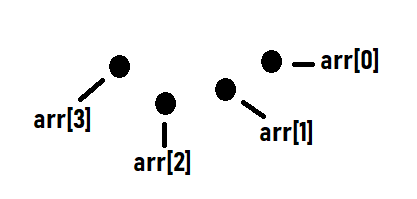
\includegraphics[scale=0.7]{titikUlar}  
	\caption[Koordinat bagian tubuh ular pada array]{Koordinat bagian tubuh ular pada array}
	\label{fig:titikUlar} 
\end{figure}

\begin{figure}[H]
	\centering  
	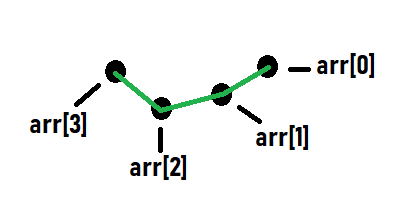
\includegraphics[scale=0.7]{garisUlar}  
	\caption[Tubuh ular setelah digambar menggunakan garis]{Tubuh ular setelah digambar menggunakan garis}
	\label{fig:garisUlar} 
\end{figure}

Untuk membuat apel digunakan \textit{quadratic Bezier curve}. Untuk memudahkan penggambaran, apel akan dianggap sebagai objek yang berbentuk persegi. 

\subsubsection{Pergerakan Ular}
Pada permainan ini, ular digerakan dengan menggunakan tombol pada keyboard. Tombol ke kiri akan membuat ular bergerak melawan arah jarum jam dan tombol ke kanan akan membuat ular akan bergerak searah jarum jam. Gambar~\ref{fig:pergerakanUlar} menunjukan pergerakan ular. 

\begin{figure}[H]
	\centering  
	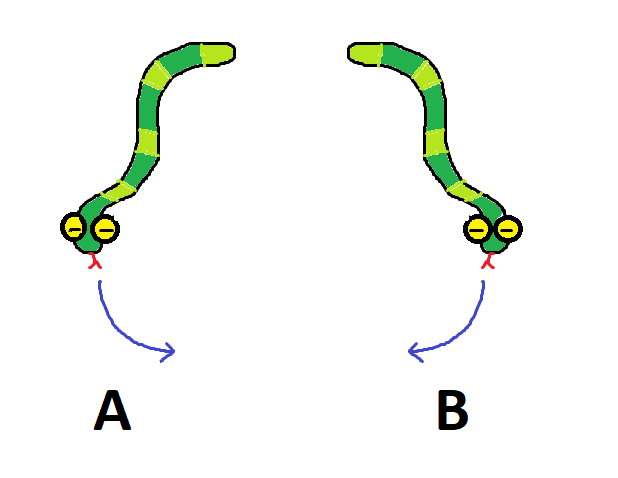
\includegraphics[scale=0.5]{pergerakanUlar}  
	\caption[Pergerakan ular (A) melawan arah jarum jam dan (B) searah jarum jam]{Pergerakan ular (A) melawan arah jarum jam dan (B) searah jarum jam}
	\label{fig:pergerakanUlar} 
\end{figure}



\subsubsection{Labirin}


\section{Analisis Berorientasi Objek}

\subsection{Diagram \textit{Use Case}}
Pada bagian ini akan dijelaskan dan ditunjukkan diagram \textit{use case} dari permainan \textit{Snake} 360. Penjelasan meliputi skenario, aktor, prakondisi skenario normal dan eksepsi. Aktor yang melakukanya adalah pemain. Pada Gambar~\ref{fig:useCase} terdapat diagram use case dari permainan \textit{Snake} 360.

\begin{figure}[H]
	\centering  
	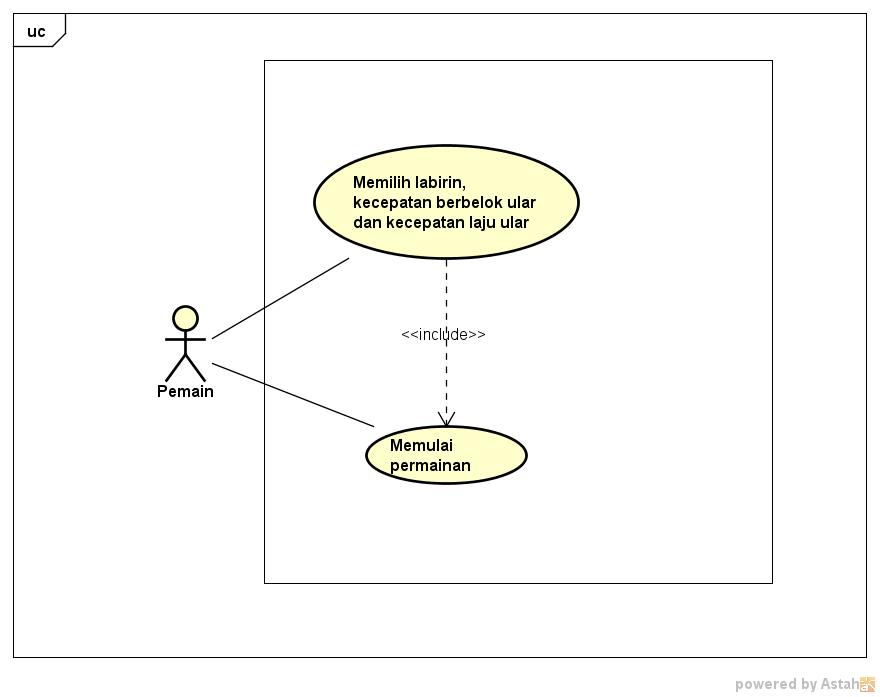
\includegraphics[scale=0.4]{useCase}  
	\caption[Diagram use case dari permainan Snake 360]{Diagram use case dari permainan Snake 360}
	\label{fig:useCase} 
\end{figure}

Berikut adalah skenario dari diagram \textit{use case} :

\begin{enumerate}
	\item Skenario : Mulai bermain \\
Aktor : Pemain \\
Prakondisi : Pemain memulai permainan.\\
Skenario normal : Pemain memulai bermain. Setelah memilih, pemain akan memilih level dan labirin. \\
Eksepsi : - \\

	\item Skenario : Memilih level dan labirin \\
Aktor : Pemain \\
Prakondisi : Pemain sudah mulai bermain. \\
Skenario normal : Pemain memilih level dan labirin yang diinginkan. \\ 
Eksepsi : - \\
\end{enumerate}

\subsection{Diagram Kelas}
Pada Gambar~\ref{fig:classDiagram} terdapat diagram kelas dari Snake 360.

\begin{figure}[H]
	\centering  
	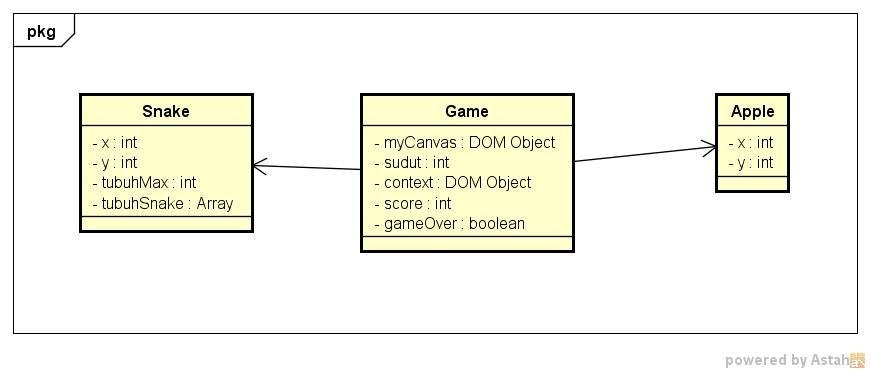
\includegraphics[scale=0.4]{classDiagram}  
	\caption[Diagram class dari permainan Snake 360]{Diagram kelas dari permainan Snake 360}
	\label{fig:classDiagram} 
\end{figure}

Diagram kelas terdiri dari beberapa kelas yaitu :

\begin{enumerate}
	\item Kelas Snake merupakan  kelas yang merepresentasikan objek ular.
	\item Kelas Apel merupakan kelas yang merepresentasikan objek apel.
	\item Kelas Game merupakan kelas yang mengatur jalanya permainan.
\end{enumerate}

Berikut adalah atribut yang dimiliki setiap kelas :

\begin{enumerate}
	\item Kelas Snake\\
\textbf{int}

\begin{itemize}
	\item x, merupakan posisi ular pada koordinat x
	\item y, merupakan posisi ular pada koordinat y
	\item tubuhMax, merupakan panjang tubuh ular
\end{itemize}

	\item Kelas Apel\\
	\textbf{int}
	
\begin{itemize}
	\item x, merupakan posisi apel pada koordinat x
	\item y, merupakan posisi apel pada koordinat y
\end{itemize}

\item Kelas Game \\
\textbf{int}

\begin{itemize}
	\item sudut, merupakan besar sudut yang digunakan untuk ular berbelok.
	\item score, merupakan skor yang didapat pada permainan.
\end{itemize}

\textbf{boolean}
\begin{itemize}
	\item gameOver, memberitahu apakah permainan sudah berakhir atau belum.
\end{itemize}

\end{enumerate}